\documentclass[xcolor=x11names,compress]{beamer}

%%%%%%%%%%%%%%%%%%%%%%%%%%%%%%%%%%%%%%%%%%%%%%%%%%%%%%%%%%%%%%%%%%%%%%%%%%%%%%
%%%%%%%%%%%%%%%%%%%%%%%%%%%%%%%%% PAKIETY %%%%%%%%%%%%%%%%%%%%%%%%%%%%%%%%%%%%
%%%%%%%%%%%%%%%%%%%%%%%%%%%%%%%%%%%%%%%%%%%%%%%%%%%%%%%%%%%%%%%%%%%%%%%%%%%%%%
\usepackage[utf8]{inputenc} % input encoding
\usepackage[T1]{fontenc}    % 8-bit font encoding (needed by e.g. PDFs)
\usepackage{listings}       % actual code package
\usepackage{diagbox}        % diagonal line in table header cell
\usepackage{tikz}           % draw graphs
\usepackage{mathtools}


%%%%%%%%%%%%%%%%%%%%%%%%%%%%%%%%%%%%%%%%%%%%%%%%%%%%%%%%%%%%%%%%%%%%%%%%%%%%%%
%%%%%%%%%%%%%%%%%%%%%%%%%%%%%%%%%% LAYOUT %%%%%%%%%%%%%%%%%%%%%%%%%%%%%%%%%%%%
%%%%%%%%%%%%%%%%%%%%%%%%%%%%%%%%%%%%%%%%%%%%%%%%%%%%%%%%%%%%%%%%%%%%%%%%%%%%%%
\usetikzlibrary{decorations.fractals}

\lstset{
  language={[Sharp]C},
  basicstyle=\tiny
}

\useoutertheme[subsection=false,shadow]{miniframes}
\useinnertheme{default}
\usefonttheme{serif}
\usepackage{palatino}

\setbeamerfont{title like}{shape=\scshape}
\setbeamerfont{frametitle}{shape=\scshape}

\definecolor{firebrick}{rgb}{.60, .20, .18}
\definecolor{sienna}{rgb}{.95, .82, .64}

\setbeamercolor*{title}{bg=white}
\setbeamercolor*{titlelike}{bg=sienna}
\setbeamercolor*{lower separation line head}{bg=firebrick} 
\setbeamercolor*{normal text}{fg=black,bg=white} 
\setbeamercolor*{alerted text}{fg=red} 
\setbeamercolor*{example text}{fg=black} 
\setbeamercolor*{structure}{fg=black} 
 
\setbeamercolor*{palette tertiary}{fg=black,bg=black!10} 
\setbeamercolor*{palette quaternary}{fg=black,bg=black!10} 

\renewcommand{\(}{\begin{columns}}
\renewcommand{\)}{\end{columns}}
\newcommand{\<}[1]{\begin{column}{#1}}
\renewcommand{\>}{\end{column}}


\begin{document}

%%%%%%%%%%%%%%%%%%%%%%%%%%%%%%%%%%%%%%%%%%%%%%%%%%%%%%%%%%%%%%%%%%%%%%%%%%%%%%
%%%%%%%%%%%%%%%%%%%%%%%%%%%%% STRONA TYTUŁOWA %%%%%%%%%%%%%%%%%%%%%%%%%%%%%%%%
%%%%%%%%%%%%%%%%%%%%%%%%%%%%%%%%%%%%%%%%%%%%%%%%%%%%%%%%%%%%%%%%%%%%%%%%%%%%%%
\begin{frame}
\title{Narzędzia do obliczania równowag Nasha}
\subtitle{przy pomocy biblioteki MathProg}
\author[M. Kubuszok]{
  Mateusz Kubuszok\\
  \bigskip
  \tiny{promotor}\\
  \scriptsize{dr inż. Piotr Więcek}\\
}
\institute[Politechnika Wrocławska]{
  \IfFileExists{znak-pwr_pion-pl-cmyk.eps}
               {}
               {\write18{wget http://www.logotyp.pwr.wroc.pl/img/Graph/ZnakPWr/WersjaPionowa/Files/Cmyk/znak-pwr_pion-pl-cmyk.eps}}
  \includegraphics[width=38pt, height=52pt]{znak-pwr_pion-pl-cmyk.eps}
}
\date[Lipiec 2014]{\tiny{03.07.2014r.}}
\titlepage
\end{frame}


%%%%%%%%%%%%%%%%%%%%%%%%%%%%%%%%%%%%%%%%%%%%%%%%%%%%%%%%%%%%%%%%%%%%%%%%%%%%%%
%%%%%%%%%%%%%%%%%%%%%%%%%%%%%%%% CEL PRACY %%%%%%%%%%%%%%%%%%%%%%%%%%%%%%%%%%%
%%%%%%%%%%%%%%%%%%%%%%%%%%%%%%%%%%%%%%%%%%%%%%%%%%%%%%%%%%%%%%%%%%%%%%%%%%%%%%
\section{\scshape Cel pracy}

\subsection{Cel pracy}
\begin{frame}{Cel pracy}
Narzędzia do obliczania wybranych równowag Nasha:
\begin{itemize}
\item szybkie w działaniu,
\item łatwe w utrzymaniu i rozbudowie,
\item dobrze udokumentowane.
\end{itemize}
\end{frame}

\subsection{Cel pracy}
\begin{frame}{Cel pracy}
Rozważane przypadki:
\begin{itemize}
\item gry jednomacierzowe,
\item gry dwumacierzowe,
\item gry z informacją doskonałą.
\end{itemize}
\end{frame}


%%%%%%%%%%%%%%%%%%%%%%%%%%%%%%%%%%%%%%%%%%%%%%%%%%%%%%%%%%%%%%%%%%%%%%%%%%%%%%
%%%%%%%%%%%%%%%%%%%%%%%%%%% GRY JEDNOMACIERZOWE %%%%%%%%%%%%%%%%%%%%%%%%%%%%%%
%%%%%%%%%%%%%%%%%%%%%%%%%%%%%%%%%%%%%%%%%%%%%%%%%%%%%%%%%%%%%%%%%%%%%%%%%%%%%%
\section{\scshape Gry jednomacierzowe}

\subsection{Gry jednomacierzowe}
\begin{frame}{Gry jednomacierzowe}
\begin{columns}[c]
\begin{column}{.5\textwidth}
Gra:
\begin{itemize}
\item w postaci strategicznej,
\item 2-osobowa,
\item o sumie zerowej.
\end{itemize}
\end{column}
\begin{column}{.5\textwidth}
Wypłaty w formie macierzy:
\begin{itemize}
\item wiersze $\rightarrow$ strategie 1. gracza,
\item kolumny $\rightarrow$ strategie 2. gracza,
\item wartości $\rightarrow$ wypłaty 1. gracza.
\end{itemize} 
\end{column}
\end{columns}
\end{frame}

%%%%%%%%%%%%%%%%%%%%%%%%%%%%%%%%%%%%%%%%%%%%%%%%%%%%%%%%%%%%%%%%%%%%%%%%%%%%%%

\subsection{Gry jednomacierzowe}
\begin{frame}{Gry jednomacierzowe - paper-kamień-nożyce}
\begin{columns}[c]
\begin{column}{.5\textwidth}
\begin{center}
Postać strategiczna:
\begin{tabular}[t]{| c              | c      | c      | c      |}
\hline
                     \diagbox{1}{2} & p      &  k     & n      \\
\hline
                     p              &  0,  0 &  1, -1 & -1,  1 \\
\hline
                     k              & -1,  1 &  0,  0 &  1, -1 \\
\hline
                     n              &  1, -1 & -1,  1 &  0,  0 \\
\hline
\end{tabular}
\end{center}
\begin{center}
Macierz wypłat:
\[\begin{bmatrix*}[r]
  0 &  1 & -1 \\
 -1 &  0 &  1 \\
  1 & -1 &  0 \\
\end{bmatrix*}\]
\end{center}
\end{column}
\begin{column}{.5\textwidth}
\begin{center}
\includegraphics[width=0.7\textwidth]{kps.pdf}
$$\sigma_1(p) = \sigma_1(k) = \sigma_1(n) = \frac{1}{3}$$
$$\sigma_2(p) = \sigma_2(k) = \sigma_2(n) = \frac{1}{3}$$
\end{center}
\end{column}
\end{columns}
\end{frame}

\subsection{Gry jednomacierzowe}
\begin{frame}[fragile]{Gry jednomacierzowe - paper-kamień-nożyce}
\begin{columns}[c]
\begin{column}{.5\textwidth}
\begin{lstlisting}
LET rock_paper_scissors
 BE STRATEGIC GAME
    WITH PLAYER p1 { rock, paper, scissors },
         PLAYER p2 { rock, paper, scissors }
    SUCH AS
      { p1=rock:
        { p2=rock:      0 },
        { p2=paper:     1 },
        { p2=scissors: -1 }
      },
      { p1=paper:
        { p2=rock:     -1 },
        { p2=paper:     0 },
        { p2=scissors:  1 }
      },
      { p1=scissors:
        { p2=rock:      1 },
        { p2=paper:    -1 },
        { p2=scissors:  0 }
      }
    END;

FIND pure_equilibrium,
     mixed_equilibrium
 FOR rock_paper_scissors;
\end{lstlisting}
\end{column}
\hspace{5pt}\vrule\hspace{5pt}
\begin{column}{.5\textwidth}
\begin{lstlisting}
Result:
  Param defined successfully
1:
  pure_equilibrium:
    No Nash equilibrium found
  mixed_equilibrium:
    Mixed Strategies:
      p1:
        rock:
          0.33333
        paper:
          0.33333
        scissors:
          0.33333
      p2:
        rock:
          0.33333
        paper:
          0.33333
        scissors:
          0.33333
    Payoff:
          p1,       p2
      Payoff:
          0.00000,  -0.00000
\end{lstlisting}
\end{column}
\end{columns}
\end{frame}


%%%%%%%%%%%%%%%%%%%%%%%%%%%%%%%%%%%%%%%%%%%%%%%%%%%%%%%%%%%%%%%%%%%%%%%%%%%%%%
%%%%%%%%%%%%%%%%%%%%%%%%%%%% GRY DWUMACIERZOWE %%%%%%%%%%%%%%%%%%%%%%%%%%%%%%%
%%%%%%%%%%%%%%%%%%%%%%%%%%%%%%%%%%%%%%%%%%%%%%%%%%%%%%%%%%%%%%%%%%%%%%%%%%%%%%
\section{\scshape Gry dwumacierzowe}

\subsection{Gry dwumacierzowe}
\begin{frame}{Gry dwumacierzowe}
\begin{columns}[c]
\begin{column}{.5\textwidth}
Gra:
\begin{itemize}
\item w postaci strategicznej,
\item 2-osobowa,
\item o sumie dowolnej.
\end{itemize}
\end{column}
\begin{column}{.5\textwidth}
Wypłaty w formie dwóch macierzy:
\begin{itemize}
\item wiersze $\rightarrow$ strategie 1. gracza,
\item kolumny $\rightarrow$ strategie 2. gracza,
\item wartości 1. macierzy $\rightarrow$ wypłaty 1 gracza,
\item wartości 2. macierzy $\rightarrow$ wypłaty 2 gracza.
\end{itemize} 
\end{column}
\end{columns}
\end{frame}

%%%%%%%%%%%%%%%%%%%%%%%%%%%%%%%%%%%%%%%%%%%%%%%%%%%%%%%%%%%%%%%%%%%%%%%%%%%%%%

\subsection{Gry dwumacierzowe}
\begin{frame}{Gry dwumacierzowe - dylemat więźnia}
\begin{columns}[c]
\begin{column}{.5\textwidth}
\begin{center}
Postać strategiczna:
\begin{tabular}[t]{| c              | c      | c               |}
\hline
                     \diagbox{1}{2} & c      & d               \\
\hline
                     c              & -1, -1 & -3,  0          \\
\hline
                     d              &  0, -3 & \textbf{-2, -2} \\
\hline
\end{tabular}
\end{center}
\end{column}
\begin{column}{.5\textwidth}
\begin{center}
Macierze wypłat:
\[\begin{bmatrix*}[r]
 -1 & -3 \\
  0 & -2 \\
\end{bmatrix*}\]
\[\begin{bmatrix*}[r]
 -1 &  0 \\
 -3 & -2 \\
\end{bmatrix*}\]
\end{center}
\end{column}
\end{columns}
\end{frame}

\subsection{Gry dwumacierzowe}
\begin{frame}[fragile]{Gry dwumacierzowe - dylemat więźnia}
\begin{columns}[c]
\begin{column}{.5\textwidth}
\begin{lstlisting}
LET prisoners_dilemma
 BE STRATEGIC GAME
    WITH PLAYER p1 { cooperates, defects },
         PLAYER p2 { cooperates, defects }
    SUCH AS
      { p1=cooperates:
        { p2=cooperates: -1, -1 },
        { p2=defects:    -3,  0 }
      },
      { p1=defects:
        { p2=cooperates:  0, -3 },
        { p2=defects:    -2, -2 }
      }
    END;

FIND pure_equilibrium,
     mixed_equilibrium
 FOR prisoners_dilemma;
\end{lstlisting}
\end{column}
\hspace{5pt}\vrule\hspace{5pt}
\begin{column}{.5\textwidth}
\begin{lstlisting}
Result:
  Param defined successfully
1:
  pure_equilibrium:
    Pure Strategies:
      p1:
        defects
      p2:
        defects
    Payoff:
          p1,        p2
      Payoff:
          -2.00000,  -2.00000
  mixed_equilibrium:
    Mixed Strategies:
      p1:
        cooperates:
          0.00000
        defects:
          1.00000
      p2:
        cooperates:
          0.00000
        defects:
          1.00000
    Payoff:
          p1,        p2
      Payoff:
          -2.00000,  -2.00000
\end{lstlisting}
\end{column}
\end{columns}
\end{frame}

%%%%%%%%%%%%%%%%%%%%%%%%%%%%%%%%%%%%%%%%%%%%%%%%%%%%%%%%%%%%%%%%%%%%%%%%%%%%%%

\subsection{Gry dwumacierzowe}
\begin{frame}{Gry dwumacierzowe - bitwa płci}
\begin{columns}[c]
\begin{column}{.5\textwidth}
\begin{center}
Postać strategiczna:
\begin{tabular}[t]{| c              | c             | c             |}
\hline
                     \diagbox{1}{2} & p             & f             \\
\hline
                     o              & \textbf{3, 2} & 0, 0          \\
\hline
                     f              & 0, 0          & \textbf{2, 3} \\
\hline
\end{tabular}
\end{center}
\end{column}
\begin{column}{.5\textwidth}
\begin{center}
Macierze wypłat:
\[\begin{bmatrix}
 3 & 0 \\
 0 & 2 \\
\end{bmatrix}\]
\[\begin{bmatrix}
 2 & 0 \\
 0 & 3 \\
\end{bmatrix}\]
\end{center}
\end{column}
\end{columns}
\end{frame}

\subsection{Gry dwumacierzowe}
\begin{frame}[fragile]{Gry dwumacierzowe - bitwa płci}
\begin{columns}[c]
\begin{column}{.5\textwidth}
\begin{lstlisting}
LET battle_of_the_sexes
 BE STRATEGIC GAME
    WITH PLAYER w { opera, football },
         PLAYER h { opera, football }
    SUCH AS
      { w=opera:
        { h=opera:    3, 2 },
        { h=football: 0, 0 }
      },
      { w=football:
        { h=opera:    0, 0 },
        { h=football: 2, 3 }
      }
    END;
    
FIND pure_equilibrium,
     mixed_equilibrium
 FOR battle_of_the_sexes;
\end{lstlisting}
\end{column}
\hspace{5pt}\vrule\hspace{5pt}
\begin{column}{.5\textwidth}
\begin{lstlisting}
Result:
  Param defined successfully
1:
  pure_equilibrium:
    Pure Strategies:
      h:
        opera
      w:
        opera
    Payoff:
          h,        w
      Payoff:
          3.00000,  2.00000
  mixed_equilibrium:
    Mixed Strategies:
      h:
        opera:
          0.60000
        football:
          0.40000
      w:
        opera:
          0.40000
        football:
          0.60000
    Payoff:
          h,        w
      Payoff:
          1.20000,  1.20000
\end{lstlisting}
\end{column}
\end{columns}
\end{frame}


%%%%%%%%%%%%%%%%%%%%%%%%%%%%%%%%%%%%%%%%%%%%%%%%%%%%%%%%%%%%%%%%%%%%%%%%%%%%%%
%%%%%%%%%%%%%%%%%%%%%%%%% GRY Z INFORMACJĄ PEŁNĄ %%%%%%%%%%%%%%%%%%%%%%%%%%%%%
%%%%%%%%%%%%%%%%%%%%%%%%%%%%%%%%%%%%%%%%%%%%%%%%%%%%%%%%%%%%%%%%%%%%%%%%%%%%%%
\section{\scshape Gry z informacją pełną}

\subsection{Gry z informacją pełną}
\begin{frame}{Gry z informacją pełną}
\begin{columns}[c]
\begin{column}{.5\textwidth}
Gra:
\begin{itemize}
\item w postaci ekstensywnej,
\item 1-elementowe zbiory informacyjne,
\item gwarantowane istnienie NE.
\end{itemize}
\end{column}
\begin{column}{.5\textwidth}
Reprezentowana przy pomocy drzewa:
\begin{itemize}
\item wierzchołki $\rightarrow$ wybór ruchu,
\item krawędzie $\rightarrow$ ruchy graczy,
\item liście $\rightarrow$ koniec gry - wypłata,
\item zb. informacyjny $\rightarrow$ wiedza gracza.
\end{itemize}
\end{column}
\end{columns}
\end{frame}

%%%%%%%%%%%%%%%%%%%%%%%%%%%%%%%%%%%%%%%%%%%%%%%%%%%%%%%%%%%%%%%%%%%%%%%%%%%%%%

\subsection{Gry z informacją pełną}
\begin{frame}[fragile]{Gry z informacją pełną - ultimatum}
\begin{center}
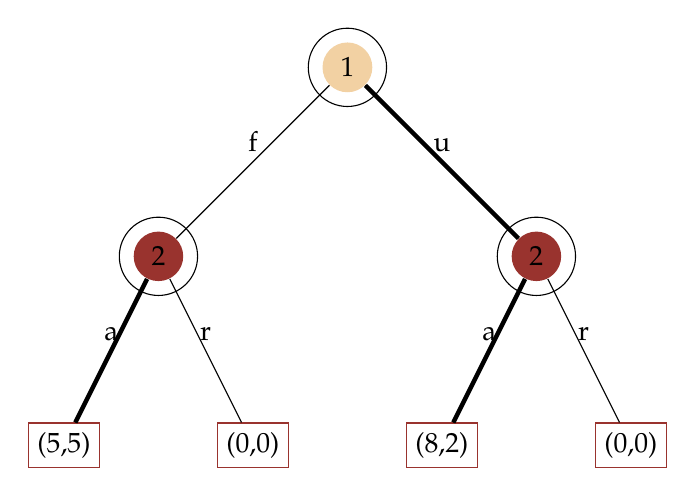
\begin{tikzpicture}[scale=.6,auto=left]
  \tikzset{IS/.style={circle, draw=black,scale=3}}
  \tikzset{P1/.style={circle, fill=sienna}}
  \tikzset{P2/.style={circle, fill=firebrick}}
  \tikzset{R/.style={draw=firebrick}}
  \node [P1] (n1)   at (0,8)  {1};
  \node [IS] (n1is) at (0,8)  {};
  \node [P2] (n2)   at (-4,4) {2};
  \node [IS] (n2is) at (-4,4) {};
  \node [P2] (n3)   at (4,4)  {2};
  \node [IS] (n3is) at (4,4)  {};
  \node [R]  (n4)   at (-6,0) {(5,5)};
  \node [R]  (n5)   at (-2,0) {(0,0)};
  \node [R]  (n6)   at (2,0)  {(8,2)};
  \node [R]  (n7)   at (6,0)  {(0,0)};

  \foreach \from/\to in {n1/n2}
    \draw (\from) -- node [above] {f} (\to);
  \foreach \from/\to in {n1/n3}
    \draw (\from) -- node [above] {u} (\to);
  \foreach \from/\to in {n2/n4,n3/n6}
    \draw (\from) -- node [above] {a} (\to);
  \foreach \from/\to in {n2/n5,n3/n7}
    \draw (\from) -- node [above] {r} (\to);
    
  \tikzset{NE/.style={ultra thick}}
  \foreach \from/\to in {n1/n3,n2/n4,n3/n6}
    \draw[NE] (\from) -- (\to);
\end{tikzpicture}
\end{center}
\end{frame}

\subsection{Gry z informacją pełną}
\begin{frame}[fragile]{Gry z informacją pełną - ultimatum}
\begin{columns}[c]
\begin{column}{.5\textwidth}
\begin{lstlisting}
LET ultimatum_game
 BE EXTENSIVE GAME
    WITH PLAYER p1 { fair,   unfair },
         PLAYER p2 { accept, reject }
    SUCH AS
      { p1=fair:
        { p2=accept: 5, 5 },
        { p2=reject: 0, 0 }
      },
      { p1=unfair:
        { p2=accept: 8, 2 },
        { p2=reject: 0, 0 }
      }
    END;

FIND pure_equilibrium
 FOR ultimatum_game;
\end{lstlisting}
\end{column}
\hspace{5pt}\vrule\hspace{5pt}
\begin{column}{.5\textwidth}
\begin{lstlisting}
Result:
  Param defined successfully
1:
  pure_equilibrium:
    Pure Strategies:
      p1:
        1:
          unfair
      p2:
        1:
          accept
        2:
          accept
    Payoff:
          p1,       p2
      Payoff:
          8.00000,  2.00000
\end{lstlisting}
\end{column}
\end{columns}
\end{frame}


%%%%%%%%%%%%%%%%%%%%%%%%%%%%%%%%%%%%%%%%%%%%%%%%%%%%%%%%%%%%%%%%%%%%%%%%%%%%%%
%%%%%%%%%%%%%%%%%%%%%%%%%%%%%% PODSUMOWANIE %%%%%%%%%%%%%%%%%%%%%%%%%%%%%%%%%%
%%%%%%%%%%%%%%%%%%%%%%%%%%%%%%%%%%%%%%%%%%%%%%%%%%%%%%%%%%%%%%%%%%%%%%%%%%%%%%
\section{\scshape Podsumowanie}

\subsection{Podsumowanie}
\begin{frame}{Podsumowanie}
\begin{center}
\textbf{Podsumowanie}
\begin{itemize}
\item projekt zakończony sukcesem,
\item poprawne obliczane NE w rozpatrywanych przypadkach,
\item możliwość dalszego rozszerzania funkcjonalności.
\end{itemize}
\end{center}
\end{frame}

\end{document}